\documentclass[xcolor=pdftex,dvipsnames,table]{UT}
\usepackage{graphicx}
%\usepackage[export]{adjustbox}
%\usepackage[pdftex]{graphicx}
\usepackage{texdraw,epsfig,bm}
\usepackage{amsfonts}
\usepackage{amsmath}
\usepackage{amssymb}
\usepackage{amsthm}
\usepackage{color}
\usepackage{mathrsfs}
\usepackage{tikz}
\usetikzlibrary{arrows}
%\usepackage{algorithm}
%\usepackage{algpseudocode}
\usepackage{dsfont}
\usepackage{amsmath}
\usepackage{forest}
\usepackage{subfig}


\background{1}	% choose background {1..5}
\taal{EN} 	%EN or NL

\title{Metropolis-Hastings \& Gibbs sampling for Bayesian inference}
\subtitle{Catalano, Fasano, Fengler, Legramanti, Rebaudo}
\date{\today} 

\begin{document} 

\maketitleslide

%Choose a sideway banner, choose (side1, side2, side3, side4, side5)
\setbeamertemplate{background}{
\includegraphics[width=0.1\paperwidth,height=\paperheight]{img/side4}} 

%includes the actual text of the files.

{\small 
	
\section*{Overview}
\begin{frame}{Overview}
\tableofcontents
\end{frame}
	
% DO NOT COMPILE THIS FILE DIRECTLY!
% This is included by the other .tex files.




%\section{Gibbs sampling for a hierarchical normal model} 
%
%\begin{frame}{Goal}
%	
%In the context of Bayesian inference, we show an example in which Gibbs sampling is the natural choice, since conditional posteriors are available (and simple).\\
%\vspace{0.2in}
%The bayesian analysis is taken from:\\
%Gelman, A., Carlin, J. B., Stern, H. S., Dunson, D. B., Vehtari, A., \& Rubin, D. B. (2014).\textit{ Bayesian data analysis (Vol. 2)}. %Boca Raton, FL: 
%CRC press.
%
%\end{frame}
%
%
%\begin{frame}{The data}
%
%Coagulation time in seconds for blood drawn from 24 animals randomly allocated to four different diets.\\
%
%\begin{figure}
%	\centering
%	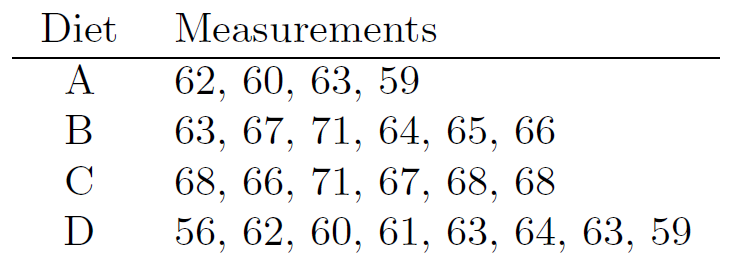
\includegraphics[width=0.7\columnwidth]{images/hier_data.png}
%\end{figure}
%
%From Box, G. E., Hunter, W. G., \& Hunter, J. S. (1978). \textit{Statistics for experimenters: an introduction to design, data analysis, and model building (Vol. 1)}. New York: Wiley.
%
%\end{frame}
%
%
%\begin{frame}{Model, prior and joint posterior}
%
%Hierarchical model:
%\begin{align*}
%y_{ij} \mid \theta, \sigma &\sim N(\theta_j,\sigma^2) \quad \quad \quad i=1, \ldots, n_j \quad \quad  j=1,\ldots, J \\
%\theta_j \mid \mu, \tau &\sim N(\mu,\tau^2) \\
%\end{align*}
%
%Prior:\\
%\vspace{0.1in}
%$\quad \quad p(\mu, \log\sigma, \log\tau) \propto \tau $\\
%\vspace{0.2in}
%Joint posterior:\\
%\vspace{0.1in}
%$\displaystyle p(\theta,\mu,\log\sigma,\log\tau \mid y) \propto \tau \prod_{j=1}^J N(\theta_j \mid \mu,\tau^2) \prod_{j=1}^{J} \prod_{i=1}^{n_j} N(y_{ij} \mid \theta_j,\sigma^2)$
%
%\end{frame}
%
%
%\begin{frame}{Conditional posteriors}
%
%$\theta_j \mid \mu, \sigma, \tau, y \sim N  \left( \hat{\theta_j},V_{\theta_j} \right)  \quad \mbox{where} \quad \hat{\theta_j} = { {{1 \over \tau^2} \mu + {n_j \over \sigma^2} \bar{y}_{\cdot j} } \over {{1 \over \tau^2}+{n_j \over \sigma^2}}}, \quad V_{\theta_j}= { 1 \over {{1 \over \tau^2}+{n_j \over \sigma^2}}} $ \\
%
%$ \displaystyle \mu \mid \theta, \sigma, \tau, y \sim N \left( \hat{\mu},{\tau^2 \over J} \right) \quad \mbox{where} \quad \hat{\mu} = {1 \over J} \sum_{j=1}^{J} \theta_j $ \\
%
%$ \displaystyle \sigma^2 \mid \theta, \mu, \tau, y \sim Inv.\chi^2 \left( n,\hat{\sigma}^2 \right)  \quad \mbox{where} \quad \hat{\sigma}^2 = {1 \over n} \sum_{j=1}^{J} \sum_{i=1}^{n_j} (y_{ij}-\theta_j)^2 $ \\
%
%$ \displaystyle \tau^2 \mid \theta, \mu, \sigma, y \sim Inv.\chi^2 \left( J-1,\hat{\tau}^2 \right)  \quad \mbox{where} \quad \hat{\tau}^2 = {1 \over {J-1}} \sum_{j=1}^{J} (\theta_j-\mu)^2 $
%
%\end{frame}
%


\section{Independent MH for the mixture of two normal distributions}


\begin{frame}{The model}

The model is a mixture of two normals with fixed parameters\\
$$\mu_1=7, \quad \mu_2=10, \quad \sigma_1=\sigma_2=0.5$$
and unknown (random) mixing proportion $\delta$.\\
\vspace{.1in}
Hence the model is:
$$ y_1, \ldots, y_n \mid \delta \quad \overset{i.i.d.}{\sim} \quad \delta N(\mu_1,\sigma_1^2) + (1-\delta) N(\mu_2,\sigma_2^2)$$\\
\vspace{0.2in}
We generate a sample of size $n=100$ with $\delta=0.7$.\\
\vspace{0.1in}
We then sample from the posterior for $\delta$ with an \textbf{independent MH} using the prior as proposal distribution.\\
\vspace{0.1in}
We expect the posterior to concentrate around the ``true" value $\delta=0.7$.
 
\end{frame}


\begin{frame}{Recall: Metropolis-Hastings (MH)}
	
		\begin{enumerate}
		\item \textbf{Initialization:} Set $t=0$ and sample $x_0$ from a starting distribution
		\item \textbf{At (t+1)-th iteration:} 
			\begin{itemize}
				\item sample the candidate $x^*$ from the proposal distribution $g(\cdot \mid x_t)$
				and compute the MH ratio
				$$ R(x_t,x^*) = \frac{f(x^*)g(x_t \mid x^*)}{f(x_t)g(x^* \mid x_t)}$$
				\item sample $u \sim U(0,1)$
				\item if $u < R(x_t,x^*)$ accept $x^*$ as $x_{t+1}$
				\item else set $x_{t+1}=x_t$
			\end{itemize}
		\end{enumerate}
	
	If $g(\cdot \mid x_t) =  g(\cdot)$, we have \textit{independent MH}.\\
	\vspace{.1in}
\textbf{Here:} f = posterior, g = prior $\implies$ R = likelihood ratio.
	
\end{frame}

\begin{frame}{Results: sample paths}

We experimented with a $Beta(1,1)=U(0,1)$ and a more skewed $Beta(2,10)$ as priors. The start was fixed at $\delta_0=0.5$ for both.
\begin{figure}
	\centering
	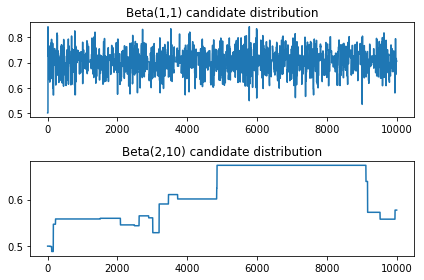
\includegraphics[width=0.5\columnwidth]{images/MCMC_chains.png}
\end{figure}
With the uniform prior, the chain moves away from $\delta_0$ quickly and explores the posterior support well (\textit{good mixing}).\\
\vspace{.1in}
With the $Beta(2,10)$ prior, only a few unique values are accepted and the mixing is poor.

\end{frame}

\begin{frame}{Results: histograms}
	
	We excluded the first 5000 iterations (\textit{burn-in}).
	\begin{figure}
		\centering
		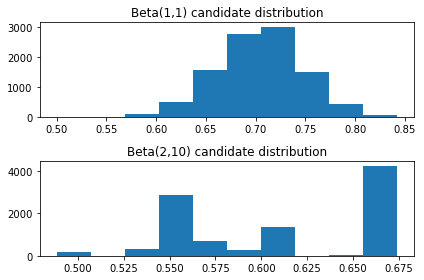
\includegraphics[width=0.5\columnwidth]{images/MCMC_hist.png}
	\end{figure}
	With the uniform prior, we get a sample with posterior mean approximately equal to 0.7, the value we used to generate the data.\\
	\vspace{.1in}
	With the $Beta(2,10)$ prior, we have already seen that we get a lot of ties and the posterior approximation is not reliable.
	
\end{frame}

 

\tikzset{>=latex}

\section{Gibbs sampling for a hierarchical normal model} 

\begin{frame}{Goal}

In the context of Bayesian inference, we show an example in which Gibbs sampling is the natural choice, since conditional posteriors are available (and simple).\\
\vspace{0.2in}
The bayesian analysis is taken from:\\
Gelman, A., Carlin, J. B., Stern, H. S., Dunson, D. B., Vehtari, A., \& Rubin, D. B. (2014).\textit{ Bayesian data analysis (Vol. 2)}. %Boca Raton, FL: 
CRC press.

\end{frame}


\begin{frame}{The data}

Coagulation time in seconds for blood drawn from 24 animals randomly allocated to four different diets.\\

\begin{figure}
\centering
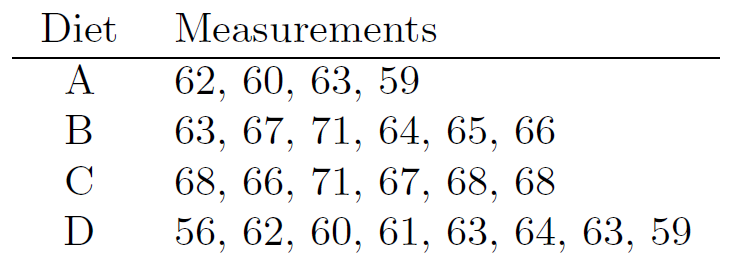
\includegraphics[width=0.7\columnwidth]{images/hier_data.png}
\end{figure}

From Box, G. E., Hunter, W. G., \& Hunter, J. S. (1978). \textit{Statistics for experimenters: an introduction to design, data analysis, and model building (Vol. 1)}. New York: Wiley.

\end{frame}

\begin{frame}{Hierarchical model}

\begin{itemize}
\item $J$ number of groups
\item $n_j$ number of observations for the group $j$
\item $y_{ji}$ $i$-th observation in group $j$ 
\item $\theta_j$ parameters for the distribution of the samples in group $j$ 
\item $\eta$ hyperparameters for the distribution of the parameters, sampled from a fixed distribution
\end{itemize}


\begin{center}
\tiny
\begin{tikzpicture}[scale=0.5]



\node [draw, thick, fill=white, shape=circle, radius=0.2cm, anchor=center, name = hyp ] at (3,5) {};
\node [draw, thick, fill=white, shape=circle, radius=0.2cm, anchor=center, name = eta ] at (3,4) {$\eta$};

\node [draw, thick, fill=white, shape=circle, radius=0.2cm, anchor=center, name = theta1 ] at (1,2) {$\theta_1$};
\node [draw, thick, fill=white, shape=circle, radius=0.2cm, anchor=center, name = theta2 ] at (2,2) {$\theta_2$};
\node [draw, thick, fill=white, shape=circle, radius=0.2cm anchor=center, name = thetaJ ] at (5,2) {$\theta_J$};

\node [draw, thick, fill=white, shape=rectangle, minimum width=0.5cm, minimum height=0.5cm, anchor=center, name = y1] at (1,0) {$y_{1\cdot}$};
\node [draw, thick, fill=white, shape=rectangle, minimum width=0.5cm, minimum height=0.5cm, anchor=center, name = y2] at (2,0) {$y_{2\cdot }$};
\node [draw, thick, fill=white, shape=rectangle, minimum width=0.5cm, minimum height=0.5cm, anchor=center, name = yJ] at (5,0) {$y_{J\cdot }$};

\draw[->] (hyp) --(eta);

\draw[->] (eta) --(theta1);
\draw[->] (eta) --(theta2);
\draw[->] (eta) --(thetaJ);

\draw[->] (theta1) --(y1);
\draw[->] (theta2) --(y2);
\draw[->] (thetaJ) --(yJ);

\node[draw] at (8,5) {Fixed distribution for the hyperparameters};
\node[draw] at (8,4) {Shared hyperparameters};
\node[draw] at (8,2) {Group parameters};
\node[draw] at (8,0) {Obervations per group};



\end{tikzpicture}
\end{center}


%\begin{flalign}
%p(y, \theta, \eta) \ & \ \propto \ p(y \mid \theta,\eta) \ p(\theta \mid \eta) \ p(\eta) \\
%& \propto \ \prod_{j=1}^J \prod_{i=1}^{n_j}  \ p(y_{ji} \mid \theta_j,\eta) \ p(\theta_j \mid \eta) \ p(\eta) \\
%\end{flalign}

\end{frame}

\begin{frame}{Hierarchical Normal Model and prior}

%Hierarchical model:

\begin{center}
\begin{forest}
	for tree={
		edge={->,>=latex},
		parent anchor=south,
		child anchor=north,
		content format={\ensuremath{\forestoption{content}}},
	}
	[{\mu,\tau},name=level0
	[\theta_{1},name=level1
	[y_{\cdot 1},name=level2]
	]
	[\theta_{2}
	[y_{\cdot 2}]
	]
	[\cdots,edge={draw=none}
	[\cdots,edge={draw=none}]
	]
	[\theta_{J}
	[y_{\cdot J}]
	]
	]
	\foreach \Name/\Label in {level2/Response variables,level1/Parameters,level0/Hyperparameters}
	\node[anchor=east] at ([xshift=-40pt]\Name) {\Label};
\end{forest}
\end{center}
\begin{align*}
y_{ij} \mid \theta, \sigma &\sim N(\theta_j,\sigma^2) \quad \quad \quad i=1, \ldots, n_j \quad \quad  j=1,\ldots, J \\
\theta_j \mid \mu, \tau &\sim N(\mu,\tau^2) \\
\end{align*}

Prior:
%\vspace{0.1in}
$\quad \quad p(\mu, \log\sigma, \log\tau) \propto \tau $\\
\vspace{0.2in}
\end{frame}


\begin{frame}{Joint and conditional posteriors}
Joint posterior:\\
\vspace{0.1in}
$\displaystyle p(\theta,\mu,\log\sigma,\log\tau \mid y) \propto \tau \prod_{j=1}^J N(\theta_j \mid \mu,\tau^2) \prod_{j=1}^{J} \prod_{i=1}^{n_j} N(y_{ij} \mid \theta_j,\sigma^2)$

Conditional posteriors:\\
\vspace{0.1in}
$\theta_j \mid \mu, \sigma, \tau, y \sim N  \left( \hat{\theta_j},V_{\theta_j} \right)  \quad \mbox{where} \quad \hat{\theta_j} = { {{1 \over \tau^2} \mu + {n_j \over \sigma^2} \bar{y}_{\cdot j} } \over {{1 \over \tau^2}+{n_j \over \sigma^2}}}, \quad V_{\theta_j}= { 1 \over {{1 \over \tau^2}+{n_j \over \sigma^2}}} $ \\

$ \displaystyle \mu \mid \theta, \sigma, \tau, y \sim N \left( \hat{\mu},{\tau^2 \over J} \right) \quad \mbox{where} \quad \hat{\mu} = {1 \over J} \sum_{j=1}^{J} \theta_j $ \\

$ \displaystyle \sigma^2 \mid \theta, \mu, \tau, y \sim Inv.\chi^2 \left( n,\hat{\sigma}^2 \right)  \quad \mbox{where} \quad \hat{\sigma}^2 = {1 \over n} \sum_{j=1}^{J} \sum_{i=1}^{n_j} (y_{ij}-\theta_j)^2 $ \\

$ \displaystyle \tau^2 \mid \theta, \mu, \sigma, y \sim Inv.\chi^2 \left( J-1,\hat{\tau}^2 \right)  \quad \mbox{where} \quad \hat{\tau}^2 = {1 \over {J-1}} \sum_{j=1}^{J} (\theta_j-\mu)^2 $

\end{frame}

\begin{frame}{The algorithm}
\begin{enumerate}
\item Fix initial values for $\hat{\theta_j}$ for $j \in \{1,\dots, J\}$. In our algorithm they are sampled from the initial data.
\item Initialize $\hat{\mu}$ with the mean of $\hat{\theta}$.
\begin{equation}
\hat{\mu} = \frac{1}{J} \sum_{j=1}^J \hat{\theta_j}
\end{equation}
\item Sample $\hat{\sigma^2}$, $\hat{\tau^2}$, $\hat{\theta_j}$, $\hat{\mu}$ from the respective conditional distributions.
\item Repeat the previous point for 1000 iterations and throw away the first half of the estimates for the parameters (warm-up).
\item Repeat from point 1 to point 4 for 10 chains.
\end{enumerate}
\end{frame}

\begin{frame}{Posterior histograms: Gibbs vs STAN}
\vspace*{-1cm}
\begin{figure}
	\centering
	\subfloat{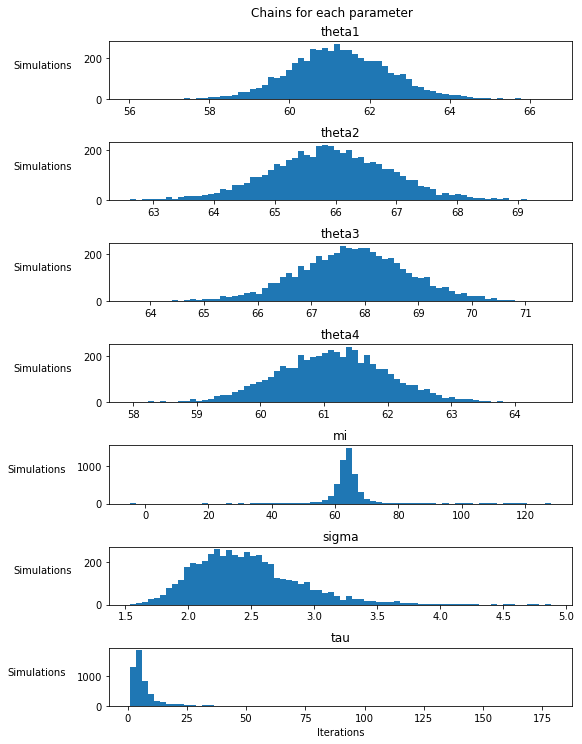
\includegraphics[width=0.5\textwidth]{images/posterior_Gibbs} }
	\subfloat{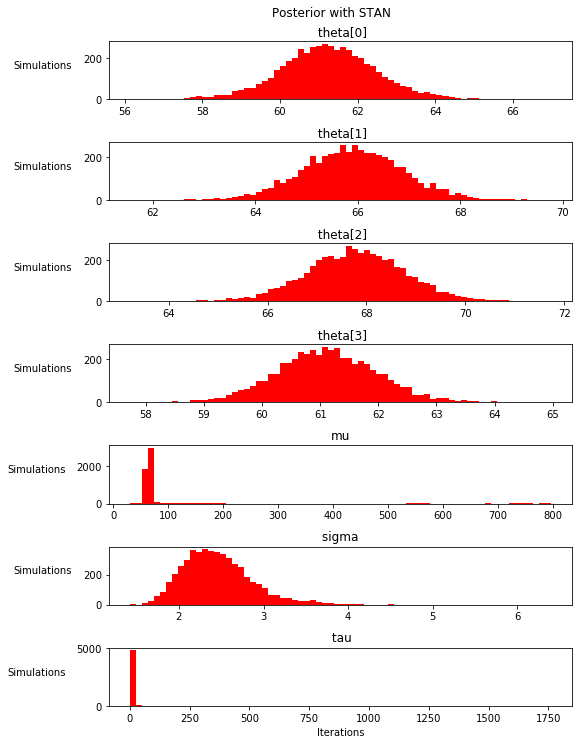
\includegraphics[width=0.5\textwidth]{images/Posterior_Stan} }
\end{figure}
\end{frame}

\begin{frame}{Runtime comparison: Gibbs vs STAN}
\vspace*{-1cm}
\begin{figure}
	\centering
	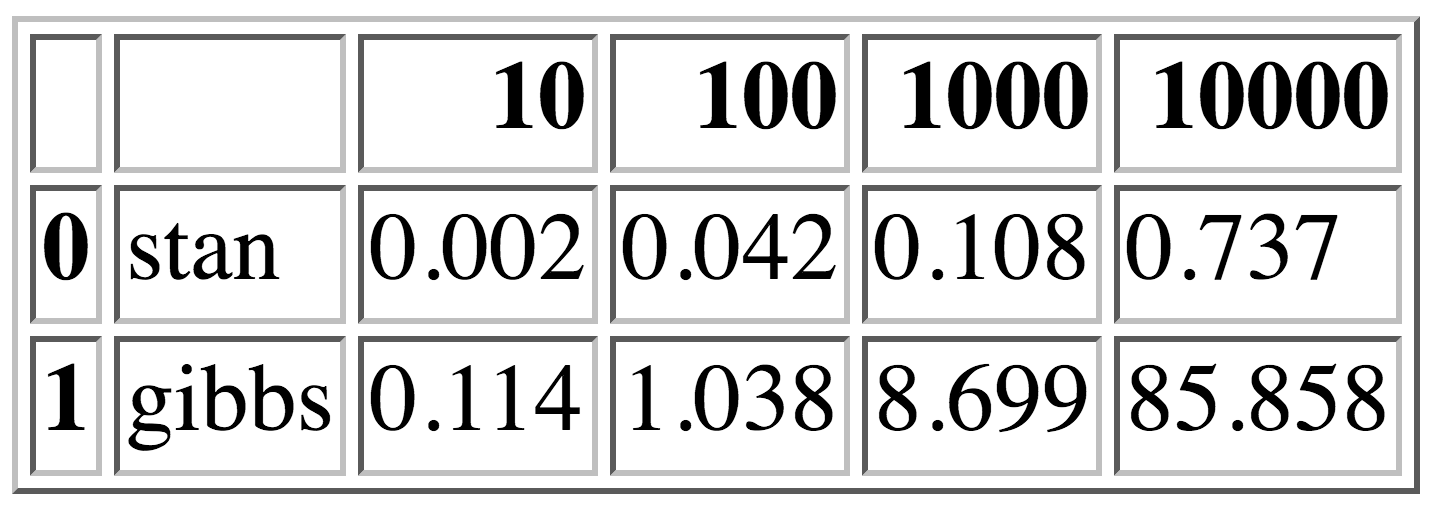
\includegraphics[width=0.7\textwidth]{images/stanvsgibbs}
\end{figure}
\end{frame}

\begin{frame}{Diagnostic}

\textbf{Problems}: \begin{itemize}
	\item early iterations reflect the starting points rather than the target distribution;
	\item within-sequence correlation can cause inefficient simulations. 
\end{itemize}
\vspace{.2in}
\textbf{Monitoring}: \begin{itemize}
	\item simulating multiple sequences with starting points dispersed in the parameters space;
	\item comparing variation intra and inter different chains.
\end{itemize}

\end{frame}


\begin{frame}{Solutions}

	\begin{itemize}
		\item For initial-values dependence, \textbf{warm-up}.\\
		The length of the warm-up should depend on the problem. Rule of thumb: discard the first half of each chain (Gelman et al.).\\
		\vspace{.2in}	
		\item For intra-chain dependence, \textbf{thinning}.\\
		Keeping only every $k$-th draw from each sequence\\
		$\Rightarrow$ storage advantages.\\
		\vspace{.2in}
		\item for both problems, \textbf{graphical comparison}.\\
	\end{itemize}	

\end{frame}

\begin{frame}{Chains}
		\centering
		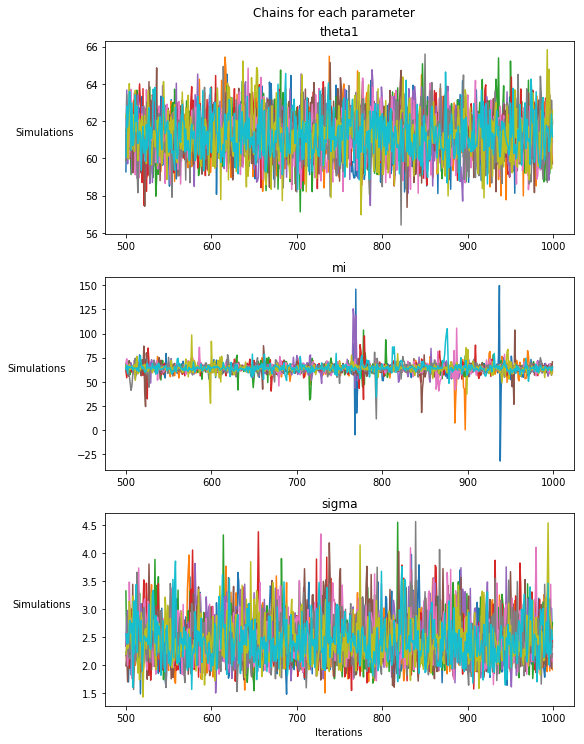
\includegraphics[width=\textwidth,height=7cm]{images/chains}
\end{frame}

\begin{frame}{Diagnostic indexes based on variance}
	We can compare the estimated variance between chains ($B$) and within chains ($W$).
	$$ B = \dfrac{n}{m-1} \sum_{j=1}^{m} (\bar{\theta}_{\cdot j} - \bar{\theta}_{\cdot \cdot})^2$$ 
	$$W = \dfrac{1}{m} \sum_{j=1}^{m} s_j^2; \,\ s_j^2 = \dfrac{1}{n-1} \sum_{i=1}^{n} (\theta_{ij} - \bar{\theta}_{\cdot j})^2$$
	$$\hat{var}(\theta|y)=\dfrac{n-1}{n} W + \dfrac{1}{n} B$$ 
	$$\hat{R} = \sqrt{\hat{var}(\theta|y)/W}$$\\
	\vspace{.1in}
	The potential scale reduction $\hat{R}$ should be closed to 1.
\end{frame}

\begin{frame}{Effective number of simulations}
Since the approximation is not based on $i.i.d.$ sample,\\
we must consider the correlation between draws.
$$N_{eff} = \dfrac{m \, n}{1+2 \sum_{t=1}^{\infty} \rho_t}$$

	\begin{center}
		\small
		\begin{tabular}{|c| c c c c c|}
			\hline	
	par & B & W & $\hat{var}$ & $\hat{R}$ & $N_{eff}$\\
	\hline	
	$\theta_1$ & 1.0032   & 1.49917 & 1.49719 & 0.999338& 4254.08\\
	$\theta_2$ & 1.21471  & 1.00384 & 1.00468 & 1.00042 & 4673.61\\
	$\theta_3$ & 2.07662  & 1.00455 & 1.00884 & 1.00213 & 4276.09\\
	$\theta_4$ & 0.912064 & 0.742049& 0.742729& 1.00046 & 4345.45\\
	$\mu$ 	   & 28.8446  & 32.1651 & 32.1518 & 0.999794& 4900.98\\
	$\sigma$   & 0.244715 & 0.164945& 0.165265& 1.00097 & 3199.1\\
	$\tau$ 	   & 203.01   & 72.0278 & 72.5517 & 1.00363 & 1605.47\\
	\hline	
		\end{tabular}
	\end{center}
\end{frame} 

\begin{frame}{}
\vspace{.5in}
\begin{center}
	Thank you for your attention!
\end{center}
\end{frame}

}

\end{document} 